\documentclass[1p]{elsarticle_modified}
%\bibliographystyle{elsarticle-num}

%\usepackage[colorlinks]{hyperref}
%\usepackage{abbrmath_seonhwa} %\Abb, \Ascr, \Acal ,\Abf, \Afrak
\usepackage{amsfonts}
\usepackage{amssymb}
\usepackage{amsmath}
\usepackage{amsthm}
\usepackage{scalefnt}
\usepackage{amsbsy}
\usepackage{kotex}
\usepackage{caption}
\usepackage{subfig}
\usepackage{color}
\usepackage{graphicx}
\usepackage{xcolor} %% white, black, red, green, blue, cyan, magenta, yellow
\usepackage{float}
\usepackage{setspace}
\usepackage{hyperref}

\usepackage{tikz}
\usetikzlibrary{arrows}

\usepackage{multirow}
\usepackage{array} % fixed length table
\usepackage{hhline}

%%%%%%%%%%%%%%%%%%%%%
\makeatletter
\renewcommand*\env@matrix[1][\arraystretch]{%
	\edef\arraystretch{#1}%
	\hskip -\arraycolsep
	\let\@ifnextchar\new@ifnextchar
	\array{*\c@MaxMatrixCols c}}
\makeatother %https://tex.stackexchange.com/questions/14071/how-can-i-increase-the-line-spacing-in-a-matrix
%%%%%%%%%%%%%%%

\usepackage[normalem]{ulem}

\newcommand{\msout}[1]{\ifmmode\text{\sout{\ensuremath{#1}}}\else\sout{#1}\fi}
%SOURCE: \msout is \stkout macro in https://tex.stackexchange.com/questions/20609/strikeout-in-math-mode

\newcommand{\cancel}[1]{
	\ifmmode
	{\color{red}\msout{#1}}
	\else
	{\color{red}\sout{#1}}
	\fi
}

\newcommand{\add}[1]{
	{\color{blue}\uwave{#1}}
}

\newcommand{\replace}[2]{
	\ifmmode
	{\color{red}\msout{#1}}{\color{blue}\uwave{#2}}
	\else
	{\color{red}\sout{#1}}{\color{blue}\uwave{#2}}
	\fi
}

\newcommand{\Sol}{\mathcal{S}} %segment
\newcommand{\D}{D} %diagram
\newcommand{\A}{\mathcal{A}} %arc


%%%%%%%%%%%%%%%%%%%%%%%%%%%%%5 test

\def\sl{\operatorname{\textup{SL}}(2,\Cbb)}
\def\psl{\operatorname{\textup{PSL}}(2,\Cbb)}
\def\quan{\mkern 1mu \triangleright \mkern 1mu}

\theoremstyle{definition}
\newtheorem{thm}{Theorem}[section]
\newtheorem{prop}[thm]{Proposition}
\newtheorem{lem}[thm]{Lemma}
\newtheorem{ques}[thm]{Question}
\newtheorem{cor}[thm]{Corollary}
\newtheorem{defn}[thm]{Definition}
\newtheorem{exam}[thm]{Example}
\newtheorem{rmk}[thm]{Remark}
\newtheorem{alg}[thm]{Algorithm}

\newcommand{\I}{\sqrt{-1}}
\begin{document}

%\begin{frontmatter}
%
%\title{Boundary parabolic representations of knots up to 8 crossings}
%
%%% Group authors per affiliation:
%\author{Yunhi Cho} 
%\address{Department of Mathematics, University of Seoul, Seoul, Korea}
%\ead{yhcho@uos.ac.kr}
%
%
%\author{Seonhwa Kim} %\fnref{s_kim}}
%\address{Center for Geometry and Physics, Institute for Basic Science, Pohang, 37673, Korea}
%\ead{ryeona17@ibs.re.kr}
%
%\author{Hyuk Kim}
%\address{Department of Mathematical Sciences, Seoul National University, Seoul 08826, Korea}
%\ead{hyukkim@snu.ac.kr}
%
%\author{Seokbeom Yoon}
%\address{Department of Mathematical Sciences, Seoul National University, Seoul, 08826,  Korea}
%\ead{sbyoon15@snu.ac.kr}
%
%\begin{abstract}
%We find all boundary parabolic representation of knots up to 8 crossings.
%
%\end{abstract}
%\begin{keyword}
%    \MSC[2010] 57M25 
%\end{keyword}
%
%\end{frontmatter}

%\linenumbers
%\tableofcontents
%
\newcommand\colored[1]{\textcolor{white}{\rule[-0.35ex]{0.8em}{1.4ex}}\kern-0.8em\color{red} #1}%
%\newcommand\colored[1]{\textcolor{white}{ #1}\kern-2.17ex	\textcolor{white}{ #1}\kern-1.81ex	\textcolor{white}{ #1}\kern-2.15ex\color{red}#1	}

{\Large $\underline{12a_{0924}~(K12a_{0924})}$}

\setlength{\tabcolsep}{10pt}
\renewcommand{\arraystretch}{1.6}
\vspace{1cm}\begin{tabular}{m{100pt}>{\centering\arraybackslash}m{274pt}}
\multirow{5}{120pt}{
	\centering
	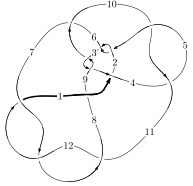
\includegraphics[width=112pt]{../../../GIT/diagram.site/Diagrams/png/1725_12a_0924.png}\\
\ \ \ A knot diagram\footnotemark}&
\allowdisplaybreaks
\textbf{Linearized knot diagam} \\
\cline{2-2}
 &
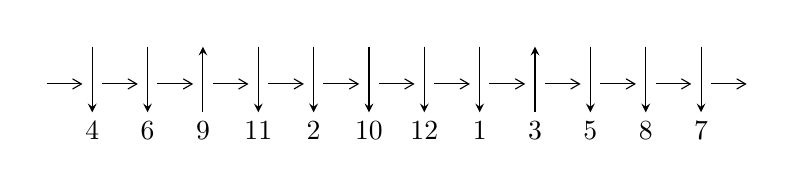
\begin{tikzpicture}[x=20pt, y=17pt]
	% nodes
	\node (C0) at (0, 0) {};
	\node (C1) at (1, 0) {};
	\node (C1U) at (1, +1) {};
	\node (C1D) at (1, -1) {4};

	\node (C2) at (2, 0) {};
	\node (C2U) at (2, +1) {};
	\node (C2D) at (2, -1) {6};

	\node (C3) at (3, 0) {};
	\node (C3U) at (3, +1) {};
	\node (C3D) at (3, -1) {9};

	\node (C4) at (4, 0) {};
	\node (C4U) at (4, +1) {};
	\node (C4D) at (4, -1) {11};

	\node (C5) at (5, 0) {};
	\node (C5U) at (5, +1) {};
	\node (C5D) at (5, -1) {2};

	\node (C6) at (6, 0) {};
	\node (C6U) at (6, +1) {};
	\node (C6D) at (6, -1) {10};

	\node (C7) at (7, 0) {};
	\node (C7U) at (7, +1) {};
	\node (C7D) at (7, -1) {12};

	\node (C8) at (8, 0) {};
	\node (C8U) at (8, +1) {};
	\node (C8D) at (8, -1) {1};

	\node (C9) at (9, 0) {};
	\node (C9U) at (9, +1) {};
	\node (C9D) at (9, -1) {3};

	\node (C10) at (10, 0) {};
	\node (C10U) at (10, +1) {};
	\node (C10D) at (10, -1) {5};

	\node (C11) at (11, 0) {};
	\node (C11U) at (11, +1) {};
	\node (C11D) at (11, -1) {8};

	\node (C12) at (12, 0) {};
	\node (C12U) at (12, +1) {};
	\node (C12D) at (12, -1) {7};
	\node (C13) at (13, 0) {};

	% arrows
	\draw[->,>={angle 60}]
	(C0) edge (C1) (C1) edge (C2) (C2) edge (C3) (C3) edge (C4) (C4) edge (C5) (C5) edge (C6) (C6) edge (C7) (C7) edge (C8) (C8) edge (C9) (C9) edge (C10) (C10) edge (C11) (C11) edge (C12) (C12) edge (C13) ;	\draw[->,>=stealth]
	(C1U) edge (C1D) (C2U) edge (C2D) (C3D) edge (C3U) (C4U) edge (C4D) (C5U) edge (C5D) (C6U) edge (C6D) (C7U) edge (C7D) (C8U) edge (C8D) (C9D) edge (C9U) (C10U) edge (C10D) (C11U) edge (C11D) (C12U) edge (C12D) ;
	\end{tikzpicture} \\
\hhline{~~} \\& 
\textbf{Solving Sequence} \\ \cline{2-2} 
 &
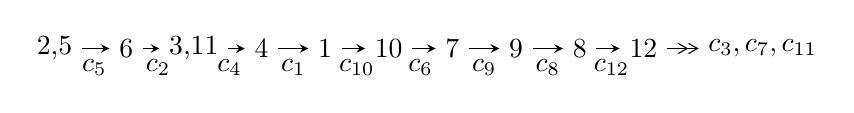
\begin{tikzpicture}[x=23pt, y=7pt]
	% node
	\node (A0) at (-1/8, 0) {2,5};
	\node (A1) at (1, 0) {6};
	\node (A2) at (33/16, 0) {3,11};
	\node (A3) at (25/8, 0) {4};
	\node (A4) at (33/8, 0) {1};
	\node (A5) at (41/8, 0) {10};
	\node (A6) at (49/8, 0) {7};
	\node (A7) at (57/8, 0) {9};
	\node (A8) at (65/8, 0) {8};
	\node (A9) at (73/8, 0) {12};
	\node (C1) at (1/2, -1) {$c_{5}$};
	\node (C2) at (3/2, -1) {$c_{2}$};
	\node (C3) at (21/8, -1) {$c_{4}$};
	\node (C4) at (29/8, -1) {$c_{1}$};
	\node (C5) at (37/8, -1) {$c_{10}$};
	\node (C6) at (45/8, -1) {$c_{6}$};
	\node (C7) at (53/8, -1) {$c_{9}$};
	\node (C8) at (61/8, -1) {$c_{8}$};
	\node (C9) at (69/8, -1) {$c_{12}$};
	\node (A10) at (11, 0) {$c_{3},c_{7},c_{11}$};

	% edge
	\draw[->,>=stealth]	
	(A0) edge (A1) (A1) edge (A2) (A2) edge (A3) (A3) edge (A4) (A4) edge (A5) (A5) edge (A6) (A6) edge (A7) (A7) edge (A8) (A8) edge (A9) ;
	\draw[->>,>={angle 60}]	
	(A9) edge (A10);
\end{tikzpicture} \\ 

\end{tabular} \\

\footnotetext{
The image of knot diagram is generated by the software ``\textbf{Draw programme}" developed by Andrew Bartholomew(\url{http://www.layer8.co.uk/maths/draw/index.htm\#Running-draw}), where we modified some parts for our purpose(\url{https://github.com/CATsTAILs/LinksPainter}).
}\phantom \\ \newline 
\centering \textbf{Ideals for irreducible components\footnotemark of $X_{\text{par}}$} 
 
\begin{align*}
I^u_{1}&=\langle 
-47905927 u^{73}+611463177 u^{72}+\cdots+3439853568 b+11169010901668,\\
\phantom{I^u_{1}}&\phantom{= \langle  }-4109478614099 u^{73}+27248497195437 u^{72}+\cdots+29824677052416 a+129084806711241884,\\
\phantom{I^u_{1}}&\phantom{= \langle  }u^{74}-8 u^{73}+\cdots-216611 u+52022\rangle \\
I^u_{2}&=\langle 
u^3+b+2 u,\;-8 u^3-3 u^2+5 a-17 u-7,\;u^4+3 u^2+1\rangle \\
I^u_{3}&=\langle 
a^2+b- a,\;a^3-2 a^2+a+1,\;u+1\rangle \\
I^u_{4}&=\langle 
b^6 a^3-3 b^5 a^2+\cdots- a^2+1,\;u+1\rangle \\
\\
I^v_{1}&=\langle 
a,\;b^6- b^5+2 b^4-2 b^3+2 b^2-2 b+1,\;v-1\rangle \\
I^v_{2}&=\langle 
a,\;b^3+b^2+2 b+1,\;v-1\rangle \\
\end{align*}
\raggedright * 5 irreducible components of $\dim_{\mathbb{C}}=0$, with total 90 representations.\\
\raggedright * 1 irreducible components of $\dim_{\mathbb{C}}=1$ \\
\footnotetext{All coefficients of polynomials are rational numbers. But the coefficients are sometimes approximated in decimal forms when there is not enough margin.}
\newpage
\renewcommand{\arraystretch}{1}
\centering \section*{I. $I^u_{1}= \langle -4.79\times10^{7} u^{73}+6.11\times10^{8} u^{72}+\cdots+3.44\times10^{9} b+1.12\times10^{13},\;-4.11\times10^{12} u^{73}+2.72\times10^{13} u^{72}+\cdots+2.98\times10^{13} a+1.29\times10^{17},\;u^{74}-8 u^{73}+\cdots-216611 u+52022 \rangle$}
\flushleft \textbf{(i) Arc colorings}\\
\begin{tabular}{m{7pt} m{180pt} m{7pt} m{180pt} }
\flushright $a_{2}=$&$\begin{pmatrix}0\\u\end{pmatrix}$ \\
\flushright $a_{5}=$&$\begin{pmatrix}1\\0\end{pmatrix}$ \\
\flushright $a_{6}=$&$\begin{pmatrix}1\\u^2\end{pmatrix}$ \\
\flushright $a_{3}=$&$\begin{pmatrix}- u\\- u^3+u\end{pmatrix}$ \\
\flushright $a_{11}=$&$\begin{pmatrix}0.137788 u^{73}-0.913623 u^{72}+\cdots+16267.3 u-4328.12\\0.0139267 u^{73}-0.177758 u^{72}+\cdots+9142.14 u-3246.94\end{pmatrix}$ \\
\flushright $a_{4}=$&$\begin{pmatrix}-0.00499643 u^{73}+0.0350880 u^{72}+\cdots-833.787 u+264.234\\0.0000461649 u^{73}-0.000532115 u^{72}+\cdots+23.8243 u-7.51639\end{pmatrix}$ \\
\flushright $a_{1}=$&$\begin{pmatrix}0.00140672 u^{73}-0.0127174 u^{72}+\cdots+521.516 u-198.382\\-0.00563162 u^{73}+0.0396538 u^{72}+\cdots-889.693 u+268.556\end{pmatrix}$ \\
\flushright $a_{10}=$&$\begin{pmatrix}0.151715 u^{73}-1.09138 u^{72}+\cdots+25409.5 u-7575.06\\0.0139267 u^{73}-0.177758 u^{72}+\cdots+9142.14 u-3246.94\end{pmatrix}$ \\
\flushright $a_{7}=$&$\begin{pmatrix}0.00526992 u^{73}-0.0422065 u^{72}+\cdots+1460.05 u-545.028\\-0.00530723 u^{73}+0.0369747 u^{72}+\cdots-859.358 u+270.028\end{pmatrix}$ \\
\flushright $a_{9}=$&$\begin{pmatrix}-0.0114518 u^{73}+0.0715137 u^{72}+\cdots-1087.20 u+313.766\\0.103761 u^{73}-0.693948 u^{72}+\cdots+13273.7 u-3725.94\end{pmatrix}$ \\
\flushright $a_{8}=$&$\begin{pmatrix}-0.0202394 u^{73}+0.0938447 u^{72}+\cdots+1301.88 u-735.830\\-0.0939198 u^{73}+0.678803 u^{72}+\cdots-15904.3 u+4756.89\end{pmatrix}$ \\
\flushright $a_{12}=$&$\begin{pmatrix}0.0629844 u^{73}-0.398283 u^{72}+\cdots+5636.71 u-1251.79\\0.0577805 u^{73}-0.401753 u^{72}+\cdots+8772.09 u-2612.98\end{pmatrix}$\\&\end{tabular}
\flushleft \textbf{(ii) Obstruction class $= -1$}\\~\\
\flushleft \textbf{(iii) Cusp Shapes $= -\frac{143175559}{644972544} u^{73}+\frac{416881405}{286654464} u^{72}+\cdots-\frac{130085081890987}{5159780352} u+\frac{17208542618977}{2579890176}$}\\~\\
\newpage\renewcommand{\arraystretch}{1}
\flushleft \textbf{(iv) u-Polynomials at the component}\newline \\
\begin{tabular}{m{50pt}|m{274pt}}
Crossings & \hspace{64pt}u-Polynomials at each crossing \\
\hline $$\begin{aligned}c_{1}\end{aligned}$$&$\begin{aligned}
&64(64 u^{74}-128 u^{73}+\cdots-2725866 u+511569)
\end{aligned}$\\
\hline $$\begin{aligned}c_{2},c_{5}\end{aligned}$$&$\begin{aligned}
&u^{74}-8 u^{73}+\cdots-216611 u+52022
\end{aligned}$\\
\hline $$\begin{aligned}c_{3},c_{9}\end{aligned}$$&$\begin{aligned}
&27(27 u^{74}-27 u^{73}+\cdots-170 u+61)
\end{aligned}$\\
\hline $$\begin{aligned}c_{4},c_{10}\end{aligned}$$&$\begin{aligned}
&27(27 u^{74}-27 u^{73}+\cdots+208 u+61)
\end{aligned}$\\
\hline $$\begin{aligned}c_{6}\end{aligned}$$&$\begin{aligned}
&64(64 u^{74}+128 u^{73}+\cdots+1.69976\times10^{7} u+3434427)
\end{aligned}$\\
\hline $$\begin{aligned}c_{7},c_{11},c_{12}\end{aligned}$$&$\begin{aligned}
&u^{74}-4 u^{73}+\cdots-255 u+62
\end{aligned}$\\
\hline $$\begin{aligned}c_{8}\end{aligned}$$&$\begin{aligned}
&u^{74}+4 u^{73}+\cdots+777216 u+285696
\end{aligned}$\\
\hline
\end{tabular}\\~\\
\newpage\renewcommand{\arraystretch}{1}
\flushleft \textbf{(v) Riley Polynomials at the component}\newline \\
\begin{tabular}{m{50pt}|m{274pt}}
Crossings & \hspace{64pt}Riley Polynomials at each crossing \\
\hline $$\begin{aligned}c_{1}\end{aligned}$$&$\begin{aligned}
&4096\\
&\cdot(4096 y^{74}-135168 y^{73}+\cdots-338930953884 y+261702841761)
\end{aligned}$\\
\hline $$\begin{aligned}c_{2},c_{5}\end{aligned}$$&$\begin{aligned}
&y^{74}-42 y^{73}+\cdots+4426533163 y+2706288484
\end{aligned}$\\
\hline $$\begin{aligned}c_{3},c_{9}\end{aligned}$$&$\begin{aligned}
&729(729 y^{74}+43011 y^{73}+\cdots+40884 y+3721)
\end{aligned}$\\
\hline $$\begin{aligned}c_{4},c_{10}\end{aligned}$$&$\begin{aligned}
&729(729 y^{74}+28431 y^{73}+\cdots+91668 y+3721)
\end{aligned}$\\
\hline $$\begin{aligned}c_{6}\end{aligned}$$&$\begin{aligned}
&4096\\
&\cdot(4096 y^{74}-118784 y^{73}+\cdots-146351267872524 y+11795288818329)
\end{aligned}$\\
\hline $$\begin{aligned}c_{7},c_{11},c_{12}\end{aligned}$$&$\begin{aligned}
&y^{74}+66 y^{73}+\cdots+4787 y+3844
\end{aligned}$\\
\hline $$\begin{aligned}c_{8}\end{aligned}$$&$\begin{aligned}
&y^{74}-6 y^{73}+\cdots+199138738176 y+81622204416
\end{aligned}$\\
\hline
\end{tabular}\\~\\
\newpage\flushleft \textbf{(vi) Complex Volumes and Cusp Shapes}
$$\begin{array}{c|c|c}  
\text{Solutions to }I^u_{1}& \I (\text{vol} + \sqrt{-1}CS) & \text{Cusp shape}\\
 \hline 
\begin{aligned}
u &= \phantom{-}0.956855 + 0.323244 I \\
a &= \phantom{-}1.58587 - 1.46932 I \\
b &= \phantom{-}0.254516 + 0.831849 I\end{aligned}
 & -2.11972 - 1.41825 I & \phantom{-0.000000 } 0 \\ \hline\begin{aligned}
u &= \phantom{-}0.956855 - 0.323244 I \\
a &= \phantom{-}1.58587 + 1.46932 I \\
b &= \phantom{-}0.254516 - 0.831849 I\end{aligned}
 & -2.11972 + 1.41825 I & \phantom{-0.000000 } 0 \\ \hline\begin{aligned}
u &= -0.392834 + 0.936221 I \\
a &= \phantom{-}0.387039 + 1.005900 I \\
b &= -0.481180 - 0.404568 I\end{aligned}
 & -1.76313 - 1.05065 I & \phantom{-0.000000 } 0 \\ \hline\begin{aligned}
u &= -0.392834 - 0.936221 I \\
a &= \phantom{-}0.387039 - 1.005900 I \\
b &= -0.481180 + 0.404568 I\end{aligned}
 & -1.76313 + 1.05065 I & \phantom{-0.000000 } 0 \\ \hline\begin{aligned}
u &= \phantom{-}0.349178 + 0.959515 I \\
a &= \phantom{-}0.37166 - 1.52102 I \\
b &= -0.098677 + 1.279600 I\end{aligned}
 & \phantom{-}10.04650 - 1.75472 I & \phantom{-0.000000 } 0 \\ \hline\begin{aligned}
u &= \phantom{-}0.349178 - 0.959515 I \\
a &= \phantom{-}0.37166 + 1.52102 I \\
b &= -0.098677 - 1.279600 I\end{aligned}
 & \phantom{-}10.04650 + 1.75472 I & \phantom{-0.000000 } 0 \\ \hline\begin{aligned}
u &= -1.039710 + 0.243499 I \\
a &= \phantom{-}0.250091 - 0.954693 I \\
b &= -0.332462 - 0.537886 I\end{aligned}
 & \phantom{-}0.82573 + 1.48951 I & \phantom{-0.000000 } 0 \\ \hline\begin{aligned}
u &= -1.039710 - 0.243499 I \\
a &= \phantom{-}0.250091 + 0.954693 I \\
b &= -0.332462 + 0.537886 I\end{aligned}
 & \phantom{-}0.82573 - 1.48951 I & \phantom{-0.000000 } 0 \\ \hline\begin{aligned}
u &= \phantom{-}0.853927 + 0.261180 I \\
a &= -1.54106 + 2.19678 I \\
b &= -0.135462 - 0.805847 I\end{aligned}
 & \phantom{-}2.19115 + 2.07020 I & -1.61287 + 2.28344 I \\ \hline\begin{aligned}
u &= \phantom{-}0.853927 - 0.261180 I \\
a &= -1.54106 - 2.19678 I \\
b &= -0.135462 + 0.805847 I\end{aligned}
 & \phantom{-}2.19115 - 2.07020 I & -1.61287 - 2.28344 I\\
 \hline 
 \end{array}$$\newpage$$\begin{array}{c|c|c}  
\text{Solutions to }I^u_{1}& \I (\text{vol} + \sqrt{-1}CS) & \text{Cusp shape}\\
 \hline 
\begin{aligned}
u &= -0.280504 + 0.832280 I \\
a &= -0.514278 - 0.776313 I \\
b &= \phantom{-}0.682562 + 0.166619 I\end{aligned}
 & -4.77010 + 3.14743 I & -13.70473 - 3.39156 I \\ \hline\begin{aligned}
u &= -0.280504 - 0.832280 I \\
a &= -0.514278 + 0.776313 I \\
b &= \phantom{-}0.682562 - 0.166619 I\end{aligned}
 & -4.77010 - 3.14743 I & -13.70473 + 3.39156 I \\ \hline\begin{aligned}
u &= -1.141320 + 0.128617 I \\
a &= -0.208428 + 0.721747 I \\
b &= \phantom{-}0.188973 + 0.757335 I\end{aligned}
 & -2.36891 - 0.94403 I & \phantom{-0.000000 } 0 \\ \hline\begin{aligned}
u &= -1.141320 - 0.128617 I \\
a &= -0.208428 - 0.721747 I \\
b &= \phantom{-}0.188973 - 0.757335 I\end{aligned}
 & -2.36891 + 0.94403 I & \phantom{-0.000000 } 0 \\ \hline\begin{aligned}
u &= \phantom{-}1.090800 + 0.370077 I \\
a &= -1.24076 + 0.89624 I \\
b &= -0.514177 - 0.873216 I\end{aligned}
 & \phantom{-}0.85631 - 4.70807 I & \phantom{-0.000000 } 0 \\ \hline\begin{aligned}
u &= \phantom{-}1.090800 - 0.370077 I \\
a &= -1.24076 - 0.89624 I \\
b &= -0.514177 + 0.873216 I\end{aligned}
 & \phantom{-}0.85631 + 4.70807 I & \phantom{-0.000000 } 0 \\ \hline\begin{aligned}
u &= \phantom{-}0.364310 + 0.761476 I \\
a &= -0.37557 + 1.45470 I \\
b &= \phantom{-}0.204448 - 1.123950 I\end{aligned}
 & \phantom{-}3.44887 - 0.05340 I & -0.84658 + 2.45920 I \\ \hline\begin{aligned}
u &= \phantom{-}0.364310 - 0.761476 I \\
a &= -0.37557 - 1.45470 I \\
b &= \phantom{-}0.204448 + 1.123950 I\end{aligned}
 & \phantom{-}3.44887 + 0.05340 I & -0.84658 - 2.45920 I \\ \hline\begin{aligned}
u &= \phantom{-}0.191646 + 0.815527 I \\
a &= -0.59145 + 1.38561 I \\
b &= \phantom{-}0.438339 - 1.274520 I\end{aligned}
 & \phantom{-}7.47797 + 7.12202 I & -0.64413 - 4.63750 I \\ \hline\begin{aligned}
u &= \phantom{-}0.191646 - 0.815527 I \\
a &= -0.59145 - 1.38561 I \\
b &= \phantom{-}0.438339 + 1.274520 I\end{aligned}
 & \phantom{-}7.47797 - 7.12202 I & -0.64413 + 4.63750 I\\
 \hline 
 \end{array}$$\newpage$$\begin{array}{c|c|c}  
\text{Solutions to }I^u_{1}& \I (\text{vol} + \sqrt{-1}CS) & \text{Cusp shape}\\
 \hline 
\begin{aligned}
u &= -0.216626 + 0.805515 I \\
a &= \phantom{-}0.625128 + 0.613776 I \\
b &= -0.810740 - 0.031535 I\end{aligned}
 & -0.12800 + 7.13488 I & -8.36711 - 5.76742 I \\ \hline\begin{aligned}
u &= -0.216626 - 0.805515 I \\
a &= \phantom{-}0.625128 - 0.613776 I \\
b &= -0.810740 + 0.031535 I\end{aligned}
 & -0.12800 - 7.13488 I & -8.36711 + 5.76742 I \\ \hline\begin{aligned}
u &= -0.019667 + 1.177440 I \\
a &= \phantom{-}0.22341 + 1.62438 I \\
b &= -0.478486 - 1.241690 I\end{aligned}
 & \phantom{-}3.47740 - 11.84660 I & \phantom{-0.000000 } 0 \\ \hline\begin{aligned}
u &= -0.019667 - 1.177440 I \\
a &= \phantom{-}0.22341 - 1.62438 I \\
b &= -0.478486 + 1.241690 I\end{aligned}
 & \phantom{-}3.47740 + 11.84660 I & \phantom{-0.000000 } 0 \\ \hline\begin{aligned}
u &= \phantom{-}0.220938 + 0.770110 I \\
a &= \phantom{-}0.48419 - 1.33432 I \\
b &= -0.393339 + 1.167180 I\end{aligned}
 & \phantom{-}2.19132 + 3.60535 I & -4.61334 - 4.48567 I \\ \hline\begin{aligned}
u &= \phantom{-}0.220938 - 0.770110 I \\
a &= \phantom{-}0.48419 + 1.33432 I \\
b &= -0.393339 - 1.167180 I\end{aligned}
 & \phantom{-}2.19132 - 3.60535 I & -4.61334 + 4.48567 I \\ \hline\begin{aligned}
u &= \phantom{-}1.116020 + 0.448323 I \\
a &= -1.01041 + 1.01076 I \\
b &= -0.551215 - 1.123180 I\end{aligned}
 & \phantom{-}1.08886 - 4.47773 I & \phantom{-0.000000 } 0 \\ \hline\begin{aligned}
u &= \phantom{-}1.116020 - 0.448323 I \\
a &= -1.01041 - 1.01076 I \\
b &= -0.551215 + 1.123180 I\end{aligned}
 & \phantom{-}1.08886 + 4.47773 I & \phantom{-0.000000 } 0 \\ \hline\begin{aligned}
u &= -0.062871 + 1.206620 I \\
a &= -0.25251 - 1.53863 I \\
b &= \phantom{-}0.474532 + 1.147300 I\end{aligned}
 & -1.94478 - 7.53049 I & \phantom{-0.000000 } 0 \\ \hline\begin{aligned}
u &= -0.062871 - 1.206620 I \\
a &= -0.25251 + 1.53863 I \\
b &= \phantom{-}0.474532 - 1.147300 I\end{aligned}
 & -1.94478 + 7.53049 I & \phantom{-0.000000 } 0\\
 \hline 
 \end{array}$$\newpage$$\begin{array}{c|c|c}  
\text{Solutions to }I^u_{1}& \I (\text{vol} + \sqrt{-1}CS) & \text{Cusp shape}\\
 \hline 
\begin{aligned}
u &= \phantom{-}1.128650 + 0.526095 I \\
a &= \phantom{-}0.915681 - 1.068180 I \\
b &= \phantom{-}0.386717 + 1.327900 I\end{aligned}
 & \phantom{-}7.55452 - 3.52374 I & \phantom{-0.000000 } 0 \\ \hline\begin{aligned}
u &= \phantom{-}1.128650 - 0.526095 I \\
a &= \phantom{-}0.915681 + 1.068180 I \\
b &= \phantom{-}0.386717 - 1.327900 I\end{aligned}
 & \phantom{-}7.55452 + 3.52374 I & \phantom{-0.000000 } 0 \\ \hline\begin{aligned}
u &= \phantom{-}1.163190 + 0.452050 I \\
a &= \phantom{-}0.922106 - 0.983293 I \\
b &= \phantom{-}0.72737 + 1.24040 I\end{aligned}
 & -0.68826 - 8.14483 I & \phantom{-0.000000 } 0 \\ \hline\begin{aligned}
u &= \phantom{-}1.163190 - 0.452050 I \\
a &= \phantom{-}0.922106 + 0.983293 I \\
b &= \phantom{-}0.72737 - 1.24040 I\end{aligned}
 & -0.68826 + 8.14483 I & \phantom{-0.000000 } 0 \\ \hline\begin{aligned}
u &= -1.241260 + 0.141904 I \\
a &= \phantom{-}0.296574 - 0.534537 I \\
b &= -0.199203 - 0.922535 I\end{aligned}
 & \phantom{-}2.60736 - 3.89508 I & \phantom{-0.000000 } 0 \\ \hline\begin{aligned}
u &= -1.241260 - 0.141904 I \\
a &= \phantom{-}0.296574 + 0.534537 I \\
b &= -0.199203 + 0.922535 I\end{aligned}
 & \phantom{-}2.60736 + 3.89508 I & \phantom{-0.000000 } 0 \\ \hline\begin{aligned}
u &= \phantom{-}1.176930 + 0.463093 I \\
a &= -0.902180 + 1.007980 I \\
b &= -0.75759 - 1.34685 I\end{aligned}
 & \phantom{-}4.46422 - 11.80280 I & \phantom{-0.000000 } 0 \\ \hline\begin{aligned}
u &= \phantom{-}1.176930 - 0.463093 I \\
a &= -0.902180 - 1.007980 I \\
b &= -0.75759 + 1.34685 I\end{aligned}
 & \phantom{-}4.46422 + 11.80280 I & \phantom{-0.000000 } 0 \\ \hline\begin{aligned}
u &= -0.143657 + 1.278550 I \\
a &= \phantom{-}0.24276 + 1.40588 I \\
b &= -0.405638 - 1.018490 I\end{aligned}
 & -0.08646 - 2.61917 I & \phantom{-0.000000 } 0 \\ \hline\begin{aligned}
u &= -0.143657 - 1.278550 I \\
a &= \phantom{-}0.24276 - 1.40588 I \\
b &= -0.405638 + 1.018490 I\end{aligned}
 & -0.08646 + 2.61917 I & \phantom{-0.000000 } 0\\
 \hline 
 \end{array}$$\newpage$$\begin{array}{c|c|c}  
\text{Solutions to }I^u_{1}& \I (\text{vol} + \sqrt{-1}CS) & \text{Cusp shape}\\
 \hline 
\begin{aligned}
u &= \phantom{-}1.279230 + 0.234772 I \\
a &= -0.642765 - 0.276219 I \\
b &= -0.580762 - 0.124608 I\end{aligned}
 & \phantom{-}0.24329 - 4.29843 I & \phantom{-0.000000 } 0 \\ \hline\begin{aligned}
u &= \phantom{-}1.279230 - 0.234772 I \\
a &= -0.642765 + 0.276219 I \\
b &= -0.580762 + 0.124608 I\end{aligned}
 & \phantom{-}0.24329 + 4.29843 I & \phantom{-0.000000 } 0 \\ \hline\begin{aligned}
u &= \phantom{-}1.311670 + 0.369854 I \\
a &= \phantom{-}0.092483 - 0.294979 I \\
b &= \phantom{-}1.288210 - 0.094940 I\end{aligned}
 & -4.77612 - 11.28530 I & \phantom{-0.000000 } 0 \\ \hline\begin{aligned}
u &= \phantom{-}1.311670 - 0.369854 I \\
a &= \phantom{-}0.092483 + 0.294979 I \\
b &= \phantom{-}1.288210 + 0.094940 I\end{aligned}
 & -4.77612 + 11.28530 I & \phantom{-0.000000 } 0 \\ \hline\begin{aligned}
u &= \phantom{-}1.324880 + 0.364823 I \\
a &= -0.060136 + 0.199915 I \\
b &= -1.207270 + 0.187553 I\end{aligned}
 & -9.63709 - 7.30911 I & \phantom{-0.000000 } 0 \\ \hline\begin{aligned}
u &= \phantom{-}1.324880 - 0.364823 I \\
a &= -0.060136 - 0.199915 I \\
b &= -1.207270 - 0.187553 I\end{aligned}
 & -9.63709 + 7.30911 I & \phantom{-0.000000 } 0 \\ \hline\begin{aligned}
u &= -1.147840 + 0.773330 I \\
a &= \phantom{-}0.232086 + 1.254660 I \\
b &= \phantom{-}0.436399 - 0.614895 I\end{aligned}
 & -2.33044 - 1.74529 I & \phantom{-0.000000 } 0 \\ \hline\begin{aligned}
u &= -1.147840 - 0.773330 I \\
a &= \phantom{-}0.232086 - 1.254660 I \\
b &= \phantom{-}0.436399 + 0.614895 I\end{aligned}
 & -2.33044 + 1.74529 I & \phantom{-0.000000 } 0 \\ \hline\begin{aligned}
u &= \phantom{-}1.348690 + 0.354551 I \\
a &= \phantom{-}0.0290628 - 0.0464895 I \\
b &= \phantom{-}1.057490 - 0.302589 I\end{aligned}
 & -7.05936 - 3.20770 I & \phantom{-0.000000 } 0 \\ \hline\begin{aligned}
u &= \phantom{-}1.348690 - 0.354551 I \\
a &= \phantom{-}0.0290628 + 0.0464895 I \\
b &= \phantom{-}1.057490 + 0.302589 I\end{aligned}
 & -7.05936 + 3.20770 I & \phantom{-0.000000 } 0\\
 \hline 
 \end{array}$$\newpage$$\begin{array}{c|c|c}  
\text{Solutions to }I^u_{1}& \I (\text{vol} + \sqrt{-1}CS) & \text{Cusp shape}\\
 \hline 
\begin{aligned}
u &= \phantom{-}0.011995 + 0.576995 I \\
a &= -0.030862 + 0.532816 I \\
b &= \phantom{-}0.490221 - 0.663405 I\end{aligned}
 & \phantom{-}3.82003 + 1.44123 I & -2.42911 - 4.15844 I \\ \hline\begin{aligned}
u &= \phantom{-}0.011995 - 0.576995 I \\
a &= -0.030862 - 0.532816 I \\
b &= \phantom{-}0.490221 + 0.663405 I\end{aligned}
 & \phantom{-}3.82003 - 1.44123 I & -2.42911 + 4.15844 I \\ \hline\begin{aligned}
u &= \phantom{-}1.41066 + 0.30363 I \\
a &= \phantom{-}0.054757 + 0.271556 I \\
b &= \phantom{-}0.689456 - 0.390814 I\end{aligned}
 & -6.22916 - 2.87126 I & \phantom{-0.000000 } 0 \\ \hline\begin{aligned}
u &= \phantom{-}1.41066 - 0.30363 I \\
a &= \phantom{-}0.054757 - 0.271556 I \\
b &= \phantom{-}0.689456 + 0.390814 I\end{aligned}
 & -6.22916 + 2.87126 I & \phantom{-0.000000 } 0 \\ \hline\begin{aligned}
u &= -1.27089 + 0.74232 I \\
a &= -0.359829 - 1.266690 I \\
b &= -0.511628 + 0.814875 I\end{aligned}
 & -7.10664 + 2.78984 I & \phantom{-0.000000 } 0 \\ \hline\begin{aligned}
u &= -1.27089 - 0.74232 I \\
a &= -0.359829 + 1.266690 I \\
b &= -0.511628 - 0.814875 I\end{aligned}
 & -7.10664 - 2.78984 I & \phantom{-0.000000 } 0 \\ \hline\begin{aligned}
u &= -1.37156 + 0.56271 I \\
a &= \phantom{-}0.88834 + 1.25590 I \\
b &= \phantom{-}0.63563 - 1.37097 I\end{aligned}
 & -0.7782 + 17.9224 I & \phantom{-0.000000 } 0 \\ \hline\begin{aligned}
u &= -1.37156 - 0.56271 I \\
a &= \phantom{-}0.88834 - 1.25590 I \\
b &= \phantom{-}0.63563 + 1.37097 I\end{aligned}
 & -0.7782 - 17.9224 I & \phantom{-0.000000 } 0 \\ \hline\begin{aligned}
u &= -1.36978 + 0.57557 I \\
a &= -0.82799 - 1.26798 I \\
b &= -0.63976 + 1.31414 I\end{aligned}
 & -6.1011 + 13.7362 I & \phantom{-0.000000 } 0 \\ \hline\begin{aligned}
u &= -1.36978 - 0.57557 I \\
a &= -0.82799 + 1.26798 I \\
b &= -0.63976 - 1.31414 I\end{aligned}
 & -6.1011 - 13.7362 I & \phantom{-0.000000 } 0\\
 \hline 
 \end{array}$$\newpage$$\begin{array}{c|c|c}  
\text{Solutions to }I^u_{1}& \I (\text{vol} + \sqrt{-1}CS) & \text{Cusp shape}\\
 \hline 
\begin{aligned}
u &= -1.37394 + 0.59852 I \\
a &= \phantom{-}0.73720 + 1.24846 I \\
b &= \phantom{-}0.607699 - 1.232080 I\end{aligned}
 & -4.11337 + 9.11039 I & \phantom{-0.000000 } 0 \\ \hline\begin{aligned}
u &= -1.37394 - 0.59852 I \\
a &= \phantom{-}0.73720 - 1.24846 I \\
b &= \phantom{-}0.607699 + 1.232080 I\end{aligned}
 & -4.11337 - 9.11039 I & \phantom{-0.000000 } 0 \\ \hline\begin{aligned}
u &= -1.34574 + 0.68489 I \\
a &= \phantom{-}0.502680 + 1.250270 I \\
b &= \phantom{-}0.549270 - 0.995359 I\end{aligned}
 & -4.54187 + 7.58769 I & \phantom{-0.000000 } 0 \\ \hline\begin{aligned}
u &= -1.34574 - 0.68489 I \\
a &= \phantom{-}0.502680 - 1.250270 I \\
b &= \phantom{-}0.549270 + 0.995359 I\end{aligned}
 & -4.54187 - 7.58769 I & \phantom{-0.000000 } 0 \\ \hline\begin{aligned}
u &= \phantom{-}1.51230 + 0.35184 I \\
a &= \phantom{-}0.130676 - 0.429581 I \\
b &= -0.537934 + 0.676409 I\end{aligned}
 & -7.49574 + 1.47115 I & \phantom{-0.000000 } 0 \\ \hline\begin{aligned}
u &= \phantom{-}1.51230 - 0.35184 I \\
a &= \phantom{-}0.130676 + 0.429581 I \\
b &= -0.537934 - 0.676409 I\end{aligned}
 & -7.49574 - 1.47115 I & \phantom{-0.000000 } 0 \\ \hline\begin{aligned}
u &= -1.44576 + 0.60502 I \\
a &= -0.683032 - 1.047140 I \\
b &= -0.417484 + 1.229110 I\end{aligned}
 & \phantom{-}4.06899 + 8.19584 I & \phantom{-0.000000 } 0 \\ \hline\begin{aligned}
u &= -1.44576 - 0.60502 I \\
a &= -0.683032 + 1.047140 I \\
b &= -0.417484 - 1.229110 I\end{aligned}
 & \phantom{-}4.06899 - 8.19584 I & \phantom{-0.000000 } 0 \\ \hline\begin{aligned}
u &= -0.274408 + 0.263174 I \\
a &= -0.697845 + 0.975456 I \\
b &= -0.135972 + 0.391654 I\end{aligned}
 & -0.560147 + 0.862728 I & -9.95266 - 7.82530 I \\ \hline\begin{aligned}
u &= -0.274408 - 0.263174 I \\
a &= -0.697845 - 0.975456 I \\
b &= -0.135972 - 0.391654 I\end{aligned}
 & -0.560147 - 0.862728 I & -9.95266 + 7.82530 I\\
 \hline 
 \end{array}$$\newpage$$\begin{array}{c|c|c}  
\text{Solutions to }I^u_{1}& \I (\text{vol} + \sqrt{-1}CS) & \text{Cusp shape}\\
 \hline 
\begin{aligned}
u &= \phantom{-}1.58981 + 0.44139 I \\
a &= -0.230102 + 0.549729 I \\
b &= \phantom{-}0.422808 - 0.863129 I\end{aligned}
 & -1.65458 + 5.47067 I & \phantom{-0.000000 } 0 \\ \hline\begin{aligned}
u &= \phantom{-}1.58981 - 0.44139 I \\
a &= -0.230102 - 0.549729 I \\
b &= \phantom{-}0.422808 + 0.863129 I\end{aligned}
 & -1.65458 - 5.47067 I & \phantom{-0.000000 } 0 \\ \hline\begin{aligned}
u &= -0.26331 + 1.73526 I \\
a &= -0.098629 - 1.231090 I \\
b &= \phantom{-}0.154343 + 0.965654 I\end{aligned}
 & \phantom{-}8.73121 - 0.63574 I & \phantom{-0.000000 } 0 \\ \hline\begin{aligned}
u &= -0.26331 - 1.73526 I \\
a &= -0.098629 + 1.231090 I \\
b &= \phantom{-}0.154343 - 0.965654 I\end{aligned}
 & \phantom{-}8.73121 + 0.63574 I & \phantom{-0.000000 } 0\\
 \hline 
 \end{array}$$\newpage\newpage\renewcommand{\arraystretch}{1}
\centering \section*{II. $I^u_{2}= \langle u^3+b+2 u,\;-8 u^3-3 u^2+5 a-17 u-7,\;u^4+3 u^2+1 \rangle$}
\flushleft \textbf{(i) Arc colorings}\\
\begin{tabular}{m{7pt} m{180pt} m{7pt} m{180pt} }
\flushright $a_{2}=$&$\begin{pmatrix}0\\u\end{pmatrix}$ \\
\flushright $a_{5}=$&$\begin{pmatrix}1\\0\end{pmatrix}$ \\
\flushright $a_{6}=$&$\begin{pmatrix}1\\u^2\end{pmatrix}$ \\
\flushright $a_{3}=$&$\begin{pmatrix}- u\\- u^3+u\end{pmatrix}$ \\
\flushright $a_{11}=$&$\begin{pmatrix}\frac{8}{5} u^3+\frac{3}{5} u^2+\frac{17}{5} u+\frac{7}{5}\\- u^3-2 u\end{pmatrix}$ \\
\flushright $a_{4}=$&$\begin{pmatrix}\frac{4}{5} u^3-\frac{1}{5} u^2+\frac{11}{5} u-\frac{4}{5}\\1\end{pmatrix}$ \\
\flushright $a_{1}=$&$\begin{pmatrix}-\frac{2}{5} u^3+\frac{2}{5} u^2- u+\frac{6}{5}\\-\frac{1}{5} u^3-\frac{1}{5} u^2+\frac{1}{5} u-\frac{4}{5}\end{pmatrix}$ \\
\flushright $a_{10}=$&$\begin{pmatrix}\frac{3}{5} u^3+\frac{3}{5} u^2+\frac{7}{5} u+\frac{7}{5}\\- u^3-2 u\end{pmatrix}$ \\
\flushright $a_{7}=$&$\begin{pmatrix}-\frac{2}{5} u^3+\frac{2}{5} u^2- u+\frac{11}{5}\\-\frac{1}{5} u^3+\frac{4}{5} u^2-\frac{4}{5} u-\frac{4}{5}\end{pmatrix}$ \\
\flushright $a_{9}=$&$\begin{pmatrix}\frac{3}{5} u^3+\frac{8}{5} u^2+\frac{7}{5} u+\frac{12}{5}\\- u^3-3 u^2-2 u-2\end{pmatrix}$ \\
\flushright $a_{8}=$&$\begin{pmatrix}\frac{1}{5} u^3+\frac{8}{5} u^2+\frac{3}{5} u+\frac{11}{5}\\-\frac{3}{5} u^3-\frac{8}{5} u^2-\frac{7}{5} u-\frac{7}{5}\end{pmatrix}$ \\
\flushright $a_{12}=$&$\begin{pmatrix}\frac{3}{5} u^2+\frac{6}{5} u+\frac{8}{5}\\\frac{3}{5} u^3-\frac{2}{5} u^2-\frac{3}{5} u-\frac{3}{5}\end{pmatrix}$\\&\end{tabular}
\flushleft \textbf{(ii) Obstruction class $= 1$}\\~\\
\flushleft \textbf{(iii) Cusp Shapes $= -4$}\\~\\
\newpage\renewcommand{\arraystretch}{1}
\flushleft \textbf{(iv) u-Polynomials at the component}\newline \\
\begin{tabular}{m{50pt}|m{274pt}}
Crossings & \hspace{64pt}u-Polynomials at each crossing \\
\hline $$\begin{aligned}c_{1}\end{aligned}$$&$\begin{aligned}
&5(5 u^4-10 u^3+9 u^2-4 u+1)
\end{aligned}$\\
\hline $$\begin{aligned}c_{2},c_{5},c_{7}\\c_{11},c_{12}\end{aligned}$$&$\begin{aligned}
&u^4+3 u^2+1
\end{aligned}$\\
\hline $$\begin{aligned}c_{3},c_{4},c_{9}\\c_{10}\end{aligned}$$&$\begin{aligned}
&(u^2+1)^2
\end{aligned}$\\
\hline $$\begin{aligned}c_{6}\end{aligned}$$&$\begin{aligned}
&5(5 u^4+u^2+2 u+1)
\end{aligned}$\\
\hline $$\begin{aligned}c_{8}\end{aligned}$$&$\begin{aligned}
&u^4+7 u^2+1
\end{aligned}$\\
\hline
\end{tabular}\\~\\
\newpage\renewcommand{\arraystretch}{1}
\flushleft \textbf{(v) Riley Polynomials at the component}\newline \\
\begin{tabular}{m{50pt}|m{274pt}}
Crossings & \hspace{64pt}Riley Polynomials at each crossing \\
\hline $$\begin{aligned}c_{1}\end{aligned}$$&$\begin{aligned}
&25(25 y^4-10 y^3+11 y^2+2 y+1)
\end{aligned}$\\
\hline $$\begin{aligned}c_{2},c_{5},c_{7}\\c_{11},c_{12}\end{aligned}$$&$\begin{aligned}
&(y^2+3 y+1)^2
\end{aligned}$\\
\hline $$\begin{aligned}c_{3},c_{4},c_{9}\\c_{10}\end{aligned}$$&$\begin{aligned}
&(y+1)^4
\end{aligned}$\\
\hline $$\begin{aligned}c_{6}\end{aligned}$$&$\begin{aligned}
&25(25 y^4+10 y^3+11 y^2-2 y+1)
\end{aligned}$\\
\hline $$\begin{aligned}c_{8}\end{aligned}$$&$\begin{aligned}
&(y^2+7 y+1)^2
\end{aligned}$\\
\hline
\end{tabular}\\~\\
\newpage\flushleft \textbf{(vi) Complex Volumes and Cusp Shapes}
$$\begin{array}{c|c|c}  
\text{Solutions to }I^u_{2}& \I (\text{vol} + \sqrt{-1}CS) & \text{Cusp shape}\\
 \hline 
\begin{aligned}
u &= \phantom{-0.000000 -}0.618034 I \\
a &= \phantom{-}1.17082 + 1.72361 I \\
b &= \phantom{-0.000000 } -1.000000 I\end{aligned}
 & \phantom{-}0.986960\phantom{ +0.000000I} & -4.00000\phantom{ +0.000000I} \\ \hline\begin{aligned}
u &= \phantom{-0.000000 } -0.618034 I \\
a &= \phantom{-}1.17082 - 1.72361 I \\
b &= \phantom{-0.000000 -}1.000000 I\end{aligned}
 & \phantom{-}0.986960\phantom{ +0.000000I} & -4.00000\phantom{ +0.000000I} \\ \hline\begin{aligned}
u &= \phantom{-0.000000 -}1.61803 I \\
a &= -0.170820 - 1.276390 I \\
b &= \phantom{-0.000000 -}1.000000 I\end{aligned}
 & \phantom{-}8.88264\phantom{ +0.000000I} & -4.00000\phantom{ +0.000000I} \\ \hline\begin{aligned}
u &= \phantom{-0.000000 } -1.61803 I \\
a &= -0.170820 + 1.276390 I \\
b &= \phantom{-0.000000 } -1.000000 I\end{aligned}
 & \phantom{-}8.88264\phantom{ +0.000000I} & -4.00000\phantom{ +0.000000I}\\
 \hline 
 \end{array}$$\newpage\newpage\renewcommand{\arraystretch}{1}
\centering \section*{III. $I^u_{3}= \langle a^2+b- a,\;a^3-2 a^2+a+1,\;u+1 \rangle$}
\flushleft \textbf{(i) Arc colorings}\\
\begin{tabular}{m{7pt} m{180pt} m{7pt} m{180pt} }
\flushright $a_{2}=$&$\begin{pmatrix}0\\-1\end{pmatrix}$ \\
\flushright $a_{5}=$&$\begin{pmatrix}1\\0\end{pmatrix}$ \\
\flushright $a_{6}=$&$\begin{pmatrix}1\\1\end{pmatrix}$ \\
\flushright $a_{3}=$&$\begin{pmatrix}1\\0\end{pmatrix}$ \\
\flushright $a_{11}=$&$\begin{pmatrix}a\\- a^2+a\end{pmatrix}$ \\
\flushright $a_{4}=$&$\begin{pmatrix}a^2- a\\a\end{pmatrix}$ \\
\flushright $a_{1}=$&$\begin{pmatrix}a\\- a^2+a\end{pmatrix}$ \\
\flushright $a_{10}=$&$\begin{pmatrix}- a^2+2 a\\- a^2+a\end{pmatrix}$ \\
\flushright $a_{7}=$&$\begin{pmatrix}- a\\a^2- a\end{pmatrix}$ \\
\flushright $a_{9}=$&$\begin{pmatrix}a\\- a^2+a\end{pmatrix}$ \\
\flushright $a_{8}=$&$\begin{pmatrix}a\\- a^2+a\end{pmatrix}$ \\
\flushright $a_{12}=$&$\begin{pmatrix}a\\- a^2+a\end{pmatrix}$\\&\end{tabular}
\flushleft \textbf{(ii) Obstruction class $= -1$}\\~\\
\flushleft \textbf{(iii) Cusp Shapes $= -6$}\\~\\
\newpage\renewcommand{\arraystretch}{1}
\flushleft \textbf{(iv) u-Polynomials at the component}\newline \\
\begin{tabular}{m{50pt}|m{274pt}}
Crossings & \hspace{64pt}u-Polynomials at each crossing \\
\hline $$\begin{aligned}c_{1},c_{3},c_{4}\\c_{9},c_{10}\end{aligned}$$&$\begin{aligned}
&u^3+u+1
\end{aligned}$\\
\hline $$\begin{aligned}c_{2},c_{5}\end{aligned}$$&$\begin{aligned}
&(u+1)^3
\end{aligned}$\\
\hline $$\begin{aligned}c_{6}\end{aligned}$$&$\begin{aligned}
&u^3+2 u^2+u-1
\end{aligned}$\\
\hline $$\begin{aligned}c_{7},c_{8},c_{11}\\c_{12}\end{aligned}$$&$\begin{aligned}
&u^3
\end{aligned}$\\
\hline
\end{tabular}\\~\\
\newpage\renewcommand{\arraystretch}{1}
\flushleft \textbf{(v) Riley Polynomials at the component}\newline \\
\begin{tabular}{m{50pt}|m{274pt}}
Crossings & \hspace{64pt}Riley Polynomials at each crossing \\
\hline $$\begin{aligned}c_{1},c_{3},c_{4}\\c_{9},c_{10}\end{aligned}$$&$\begin{aligned}
&y^3+2 y^2+y-1
\end{aligned}$\\
\hline $$\begin{aligned}c_{2},c_{5}\end{aligned}$$&$\begin{aligned}
&(y-1)^3
\end{aligned}$\\
\hline $$\begin{aligned}c_{6}\end{aligned}$$&$\begin{aligned}
&y^3-2 y^2+5 y-1
\end{aligned}$\\
\hline $$\begin{aligned}c_{7},c_{8},c_{11}\\c_{12}\end{aligned}$$&$\begin{aligned}
&y^3
\end{aligned}$\\
\hline
\end{tabular}\\~\\
\newpage\flushleft \textbf{(vi) Complex Volumes and Cusp Shapes}
$$\begin{array}{c|c|c}  
\text{Solutions to }I^u_{3}& \I (\text{vol} + \sqrt{-1}CS) & \text{Cusp shape}\\
 \hline 
\begin{aligned}
u &= -1.00000\phantom{ +0.000000I} \\
a &= \phantom{-}1.23279 + 0.79255 I \\
b &= \phantom{-}0.341164 - 1.161540 I\end{aligned}
 & -1.64493\phantom{ +0.000000I} & -6.00000\phantom{ +0.000000I} \\ \hline\begin{aligned}
u &= -1.00000\phantom{ +0.000000I} \\
a &= \phantom{-}1.23279 - 0.79255 I \\
b &= \phantom{-}0.341164 + 1.161540 I\end{aligned}
 & -1.64493\phantom{ +0.000000I} & -6.00000\phantom{ +0.000000I} \\ \hline\begin{aligned}
u &= -1.00000\phantom{ +0.000000I} \\
a &= -0.465571\phantom{ +0.000000I} \\
b &= -0.682328\phantom{ +0.000000I}\end{aligned}
 & -1.64493\phantom{ +0.000000I} & -6.00000\phantom{ +0.000000I}\\
 \hline 
 \end{array}$$\newpage\newpage\renewcommand{\arraystretch}{1}
\centering \section*{IV. $I^u_{4}= \langle b^6 a^3-3 b^5 a^2+\cdots- a^2+1,\;u+1 \rangle$}
\flushleft \textbf{(i) Arc colorings}\\
\begin{tabular}{m{7pt} m{180pt} m{7pt} m{180pt} }
\flushright $a_{2}=$&$\begin{pmatrix}0\\-1\end{pmatrix}$ \\
\flushright $a_{5}=$&$\begin{pmatrix}1\\0\end{pmatrix}$ \\
\flushright $a_{6}=$&$\begin{pmatrix}1\\1\end{pmatrix}$ \\
\flushright $a_{3}=$&$\begin{pmatrix}1\\0\end{pmatrix}$ \\
\flushright $a_{11}=$&$\begin{pmatrix}a\\b\end{pmatrix}$ \\
\flushright $a_{4}=$&$\begin{pmatrix}- b a+1\\- b^2\end{pmatrix}$ \\
\flushright $a_{1}=$&$\begin{pmatrix}- b^2 a^2+2 b a-1\\- b^3 a+b^2-1\end{pmatrix}$ \\
\flushright $a_{10}=$&$\begin{pmatrix}b+a\\b\end{pmatrix}$ \\
\flushright $a_{7}=$&$\begin{pmatrix}- b a- a^2+1\\- b a+1\end{pmatrix}$ \\
\flushright $a_{9}=$&$\begin{pmatrix}a\\b\end{pmatrix}$ \\
\flushright $a_{8}=$&$\begin{pmatrix}- b^4 a^3+3 b^3 a^2- a^3 b^2-3 b^2 a+2 a^2 b+b\\- b^5 a^2+2 b^4 a- b^3 a^2- b^3+2 b- a\end{pmatrix}$ \\
\flushright $a_{12}=$&$\begin{pmatrix}- b^5 a^3- b^4 a^4+3 b^4 a^2-2 a^4 b^2-3 b^3 a+2 b^2 a^2+a^3 b- a^4+b^2+a^2-1\\- b^5 a^3+3 b^4 a^2-2 b^3 a^3-4 b^3 a+4 b^2 a^2- a^3 b+2 b^2-2 b a+a^2-1\end{pmatrix}$\\&\end{tabular}
\flushleft \textbf{(ii) Obstruction class $= 1$}\\~\\
\flushleft \textbf{(iii) Cusp Shapes $= 4 b^2 a-4 b+4 a-12$}\\~\\
\flushleft \textbf{(iv) u-Polynomials at the component} : It cannot be defined for a positive dimension component.\\~\\
\flushleft \textbf{(v) Riley Polynomials at the component} : It cannot be defined for a positive dimension component.\\~\\
\newpage\flushleft \textbf{(iv) Complex Volumes and Cusp Shapes}
$$\begin{array}{c|c|c} 
\text{Solution to }I^u_{4}& \I (\text{vol} + \sqrt{-1}CS) & \text{Cusp shape}\\
 \hline 
\begin{aligned}
u &= \cdots \\
a &= \cdots \\
b &= \cdots\end{aligned}
 & \phantom{-}1.37919 - 2.82812 I & -15.0195 + 0. I\\
 \hline 
 \end{array}
$$\newpage\renewcommand{\arraystretch}{1}
\centering \section*{V. $I^v_{1}= \langle a,\;b^6- b^5+2 b^4-2 b^3+2 b^2-2 b+1,\;v-1 \rangle$}
\flushleft \textbf{(i) Arc colorings}\\
\begin{tabular}{m{7pt} m{180pt} m{7pt} m{180pt} }
\flushright $a_{2}=$&$\begin{pmatrix}1\\0\end{pmatrix}$ \\
\flushright $a_{5}=$&$\begin{pmatrix}1\\0\end{pmatrix}$ \\
\flushright $a_{6}=$&$\begin{pmatrix}1\\0\end{pmatrix}$ \\
\flushright $a_{3}=$&$\begin{pmatrix}1\\0\end{pmatrix}$ \\
\flushright $a_{11}=$&$\begin{pmatrix}0\\b\end{pmatrix}$ \\
\flushright $a_{4}=$&$\begin{pmatrix}1\\- b^2\end{pmatrix}$ \\
\flushright $a_{1}=$&$\begin{pmatrix}b^2+1\\- b^4\end{pmatrix}$ \\
\flushright $a_{10}=$&$\begin{pmatrix}b\\b\end{pmatrix}$ \\
\flushright $a_{7}=$&$\begin{pmatrix}b^2+1\\b^2\end{pmatrix}$ \\
\flushright $a_{9}=$&$\begin{pmatrix}0\\b\end{pmatrix}$ \\
\flushright $a_{8}=$&$\begin{pmatrix}b^5+2 b^3+b\\1\end{pmatrix}$ \\
\flushright $a_{12}=$&$\begin{pmatrix}-2 b^5+b^4-4 b^3+3 b^2-3 b+3\\- b^5-2 b^3+b^2- b+1\end{pmatrix}$\\&\end{tabular}
\flushleft \textbf{(ii) Obstruction class $= -1$}\\~\\
\flushleft \textbf{(iii) Cusp Shapes $= 4 b^3+4 b-6$}\\~\\
\newpage\renewcommand{\arraystretch}{1}
\flushleft \textbf{(iv) u-Polynomials at the component}\newline \\
\begin{tabular}{m{50pt}|m{274pt}}
Crossings & \hspace{64pt}u-Polynomials at each crossing \\
\hline $$\begin{aligned}c_{1}\end{aligned}$$&$\begin{aligned}
&u^6+3 u^5+4 u^4+2 u^3+1
\end{aligned}$\\
\hline $$\begin{aligned}c_{2},c_{5}\end{aligned}$$&$\begin{aligned}
&u^6
\end{aligned}$\\
\hline $$\begin{aligned}c_{3},c_{4},c_{6}\\c_{9},c_{10}\end{aligned}$$&$\begin{aligned}
&u^6- u^5+2 u^4-2 u^3+2 u^2-2 u+1
\end{aligned}$\\
\hline $$\begin{aligned}c_{7},c_{11},c_{12}\end{aligned}$$&$\begin{aligned}
&(u^3+u^2+2 u+1)^2
\end{aligned}$\\
\hline $$\begin{aligned}c_{8}\end{aligned}$$&$\begin{aligned}
&(u^3- u^2+1)^2
\end{aligned}$\\
\hline
\end{tabular}\\~\\
\newpage\renewcommand{\arraystretch}{1}
\flushleft \textbf{(v) Riley Polynomials at the component}\newline \\
\begin{tabular}{m{50pt}|m{274pt}}
Crossings & \hspace{64pt}Riley Polynomials at each crossing \\
\hline $$\begin{aligned}c_{1}\end{aligned}$$&$\begin{aligned}
&y^6- y^5+4 y^4-2 y^3+8 y^2+1
\end{aligned}$\\
\hline $$\begin{aligned}c_{2},c_{5}\end{aligned}$$&$\begin{aligned}
&y^6
\end{aligned}$\\
\hline $$\begin{aligned}c_{3},c_{4},c_{6}\\c_{9},c_{10}\end{aligned}$$&$\begin{aligned}
&y^6+3 y^5+4 y^4+2 y^3+1
\end{aligned}$\\
\hline $$\begin{aligned}c_{7},c_{11},c_{12}\end{aligned}$$&$\begin{aligned}
&(y^3+3 y^2+2 y-1)^2
\end{aligned}$\\
\hline $$\begin{aligned}c_{8}\end{aligned}$$&$\begin{aligned}
&(y^3- y^2+2 y-1)^2
\end{aligned}$\\
\hline
\end{tabular}\\~\\
\newpage\flushleft \textbf{(vi) Complex Volumes and Cusp Shapes}
$$\begin{array}{c|c|c}  
\text{Solutions to }I^v_{1}& \I (\text{vol} + \sqrt{-1}CS) & \text{Cusp shape}\\
 \hline 
\begin{aligned}
v &= \phantom{-}1.00000\phantom{ +0.000000I} \\
a &= \phantom{-0.000000 } 0 \\
b &= -0.498832 + 1.001300 I\end{aligned}
 & \phantom{-}3.02413 - 2.82812 I & -2.49024 + 2.97945 I \\ \hline\begin{aligned}
v &= \phantom{-}1.00000\phantom{ +0.000000I} \\
a &= \phantom{-0.000000 } 0 \\
b &= -0.498832 - 1.001300 I\end{aligned}
 & \phantom{-}3.02413 + 2.82812 I & -2.49024 - 2.97945 I \\ \hline\begin{aligned}
v &= \phantom{-}1.00000\phantom{ +0.000000I} \\
a &= \phantom{-0.000000 } 0 \\
b &= \phantom{-}0.284920 + 1.115140 I\end{aligned}
 & -1.11345\phantom{ +0.000000I} & -9.01951 + 0. I\phantom{ +0.000000I} \\ \hline\begin{aligned}
v &= \phantom{-}1.00000\phantom{ +0.000000I} \\
a &= \phantom{-0.000000 } 0 \\
b &= \phantom{-}0.284920 - 1.115140 I\end{aligned}
 & -1.11345\phantom{ +0.000000I} & -9.01951 + 0. I\phantom{ +0.000000I} \\ \hline\begin{aligned}
v &= \phantom{-}1.00000\phantom{ +0.000000I} \\
a &= \phantom{-0.000000 } 0 \\
b &= \phantom{-}0.713912 + 0.305839 I\end{aligned}
 & \phantom{-}3.02413 - 2.82812 I & -2.49024 + 2.97945 I \\ \hline\begin{aligned}
v &= \phantom{-}1.00000\phantom{ +0.000000I} \\
a &= \phantom{-0.000000 } 0 \\
b &= \phantom{-}0.713912 - 0.305839 I\end{aligned}
 & \phantom{-}3.02413 + 2.82812 I & -2.49024 - 2.97945 I\\
 \hline 
 \end{array}$$\newpage\newpage\renewcommand{\arraystretch}{1}
\centering \section*{VI. $I^v_{2}= \langle a,\;b^3+b^2+2 b+1,\;v-1 \rangle$}
\flushleft \textbf{(i) Arc colorings}\\
\begin{tabular}{m{7pt} m{180pt} m{7pt} m{180pt} }
\flushright $a_{2}=$&$\begin{pmatrix}1\\0\end{pmatrix}$ \\
\flushright $a_{5}=$&$\begin{pmatrix}1\\0\end{pmatrix}$ \\
\flushright $a_{6}=$&$\begin{pmatrix}1\\0\end{pmatrix}$ \\
\flushright $a_{3}=$&$\begin{pmatrix}1\\0\end{pmatrix}$ \\
\flushright $a_{11}=$&$\begin{pmatrix}0\\b\end{pmatrix}$ \\
\flushright $a_{4}=$&$\begin{pmatrix}1\\- b^2\end{pmatrix}$ \\
\flushright $a_{1}=$&$\begin{pmatrix}b^2+1\\b^2- b-1\end{pmatrix}$ \\
\flushright $a_{10}=$&$\begin{pmatrix}b\\b\end{pmatrix}$ \\
\flushright $a_{7}=$&$\begin{pmatrix}b^2+1\\b^2\end{pmatrix}$ \\
\flushright $a_{9}=$&$\begin{pmatrix}0\\b\end{pmatrix}$ \\
\flushright $a_{8}=$&$\begin{pmatrix}-1\\2 b^2+2 b\end{pmatrix}$ \\
\flushright $a_{12}=$&$\begin{pmatrix}- b\\-3 b-2\end{pmatrix}$\\&\end{tabular}
\flushleft \textbf{(ii) Obstruction class $= -1$}\\~\\
\flushleft \textbf{(iii) Cusp Shapes $= -4 b^2-4 b-10$}\\~\\
\newpage\renewcommand{\arraystretch}{1}
\flushleft \textbf{(iv) u-Polynomials at the component}\newline \\
\begin{tabular}{m{50pt}|m{274pt}}
Crossings & \hspace{64pt}u-Polynomials at each crossing \\
\hline $$\begin{aligned}c_{1}\end{aligned}$$&$\begin{aligned}
&u^3+3 u^2+2 u-1
\end{aligned}$\\
\hline $$\begin{aligned}c_{2},c_{5}\end{aligned}$$&$\begin{aligned}
&u^3
\end{aligned}$\\
\hline $$\begin{aligned}c_{3},c_{4},c_{6}\\c_{7},c_{9},c_{10}\\c_{11},c_{12}\end{aligned}$$&$\begin{aligned}
&u^3+u^2+2 u+1
\end{aligned}$\\
\hline $$\begin{aligned}c_{8}\end{aligned}$$&$\begin{aligned}
&u^3- u^2+1
\end{aligned}$\\
\hline
\end{tabular}\\~\\
\newpage\renewcommand{\arraystretch}{1}
\flushleft \textbf{(v) Riley Polynomials at the component}\newline \\
\begin{tabular}{m{50pt}|m{274pt}}
Crossings & \hspace{64pt}Riley Polynomials at each crossing \\
\hline $$\begin{aligned}c_{1}\end{aligned}$$&$\begin{aligned}
&y^3-5 y^2+10 y-1
\end{aligned}$\\
\hline $$\begin{aligned}c_{2},c_{5}\end{aligned}$$&$\begin{aligned}
&y^3
\end{aligned}$\\
\hline $$\begin{aligned}c_{3},c_{4},c_{6}\\c_{7},c_{9},c_{10}\\c_{11},c_{12}\end{aligned}$$&$\begin{aligned}
&y^3+3 y^2+2 y-1
\end{aligned}$\\
\hline $$\begin{aligned}c_{8}\end{aligned}$$&$\begin{aligned}
&y^3- y^2+2 y-1
\end{aligned}$\\
\hline
\end{tabular}\\~\\
\newpage\flushleft \textbf{(vi) Complex Volumes and Cusp Shapes}
$$\begin{array}{c|c|c}  
\text{Solutions to }I^v_{2}& \I (\text{vol} + \sqrt{-1}CS) & \text{Cusp shape}\\
 \hline 
\begin{aligned}
v &= \phantom{-}1.00000\phantom{ +0.000000I} \\
a &= \phantom{-0.000000 } 0 \\
b &= -0.215080 + 1.307140 I\end{aligned}
 & \phantom{-}3.02413 + 2.82812 I & -2.49024 - 2.97945 I \\ \hline\begin{aligned}
v &= \phantom{-}1.00000\phantom{ +0.000000I} \\
a &= \phantom{-0.000000 } 0 \\
b &= -0.215080 - 1.307140 I\end{aligned}
 & \phantom{-}3.02413 - 2.82812 I & -2.49024 + 2.97945 I \\ \hline\begin{aligned}
v &= \phantom{-}1.00000\phantom{ +0.000000I} \\
a &= \phantom{-0.000000 } 0 \\
b &= -0.569840\phantom{ +0.000000I}\end{aligned}
 & -1.11345\phantom{ +0.000000I} & -9.01950\phantom{ +0.000000I}\\
 \hline 
 \end{array}$$\newpage
\newpage\renewcommand{\arraystretch}{1}
\centering \section*{ VII. u-Polynomials}
\begin{tabular}{m{50pt}|m{274pt}}
Crossings & \hspace{64pt}u-Polynomials at each crossing \\
\hline $$\begin{aligned}c_{1}\end{aligned}$$&$\begin{aligned}
&320(u^3+u+1)(u^3+3 u^2+2 u-1)(5 u^4-10 u^3+9 u^2-4 u+1)\\
&\cdot(u^6+3 u^5+4 u^4+2 u^3+1)\\
&\cdot(64 u^{74}-128 u^{73}+\cdots-2725866 u+511569)
\end{aligned}$\\
\hline $$\begin{aligned}c_{2},c_{5}\end{aligned}$$&$\begin{aligned}
&u^9(u+1)^3(u^4+3 u^2+1)(u^{74}-8 u^{73}+\cdots-216611 u+52022)
\end{aligned}$\\
\hline $$\begin{aligned}c_{3},c_{9}\end{aligned}$$&$\begin{aligned}
&27(u^2+1)^2(u^3+u+1)(u^3+u^2+2 u+1)\\
&\cdot(u^6- u^5+2 u^4-2 u^3+2 u^2-2 u+1)(27 u^{74}-27 u^{73}+\cdots-170 u+61)
\end{aligned}$\\
\hline $$\begin{aligned}c_{4},c_{10}\end{aligned}$$&$\begin{aligned}
&27(u^2+1)^2(u^3+u+1)(u^3+u^2+2 u+1)\\
&\cdot(u^6- u^5+2 u^4-2 u^3+2 u^2-2 u+1)(27 u^{74}-27 u^{73}+\cdots+208 u+61)
\end{aligned}$\\
\hline $$\begin{aligned}c_{6}\end{aligned}$$&$\begin{aligned}
&320(u^3+u^2+2 u+1)(u^3+2 u^2+u-1)(5 u^4+u^2+2 u+1)\\
&\cdot(u^6- u^5+2 u^4-2 u^3+2 u^2-2 u+1)\\
&\cdot(64 u^{74}+128 u^{73}+\cdots+16997580 u+3434427)
\end{aligned}$\\
\hline $$\begin{aligned}c_{7},c_{11},c_{12}\end{aligned}$$&$\begin{aligned}
&u^3(u^3+u^2+2 u+1)^{3}(u^4+3 u^2+1)(u^{74}-4 u^{73}+\cdots-255 u+62)
\end{aligned}$\\
\hline $$\begin{aligned}c_{8}\end{aligned}$$&$\begin{aligned}
&u^3(u^3- u^2+1)^3(u^4+7 u^2+1)(u^{74}+4 u^{73}+\cdots+777216 u+285696)
\end{aligned}$\\
\hline
\end{tabular}\newpage\renewcommand{\arraystretch}{1}
\centering \section*{ VIII. Riley Polynomials}
\begin{tabular}{m{50pt}|m{274pt}}
Crossings & \hspace{64pt}Riley Polynomials at each crossing \\
\hline $$\begin{aligned}c_{1}\end{aligned}$$&$\begin{aligned}
&102400(y^3-5 y^2+10 y-1)(y^3+2 y^2+y-1)\\
&\cdot(25 y^4-10 y^3+11 y^2+2 y+1)(y^6- y^5+4 y^4-2 y^3+8 y^2+1)\\
&\cdot(4096 y^{74}-135168 y^{73}+\cdots-338930953884 y+261702841761)
\end{aligned}$\\
\hline $$\begin{aligned}c_{2},c_{5}\end{aligned}$$&$\begin{aligned}
&y^9(y-1)^3(y^2+3 y+1)^2\\
&\cdot(y^{74}-42 y^{73}+\cdots+4426533163 y+2706288484)
\end{aligned}$\\
\hline $$\begin{aligned}c_{3},c_{9}\end{aligned}$$&$\begin{aligned}
&729(y+1)^4(y^3+2 y^2+y-1)(y^3+3 y^2+2 y-1)\\
&\cdot(y^6+3 y^5+4 y^4+2 y^3+1)(729 y^{74}+43011 y^{73}+\cdots+40884 y+3721)
\end{aligned}$\\
\hline $$\begin{aligned}c_{4},c_{10}\end{aligned}$$&$\begin{aligned}
&729(y+1)^4(y^3+2 y^2+y-1)(y^3+3 y^2+2 y-1)\\
&\cdot(y^6+3 y^5+4 y^4+2 y^3+1)(729 y^{74}+28431 y^{73}+\cdots+91668 y+3721)
\end{aligned}$\\
\hline $$\begin{aligned}c_{6}\end{aligned}$$&$\begin{aligned}
&102400(y^3-2 y^2+5 y-1)(y^3+3 y^2+2 y-1)\\
&\cdot(25 y^4+10 y^3+11 y^2-2 y+1)(y^6+3 y^5+4 y^4+2 y^3+1)\\
&\cdot(4096 y^{74}-118784 y^{73}+\cdots-146351267872524 y+11795288818329)
\end{aligned}$\\
\hline $$\begin{aligned}c_{7},c_{11},c_{12}\end{aligned}$$&$\begin{aligned}
&y^3(y^2+3 y+1)^2(y^3+3 y^2+2 y-1)^3\\
&\cdot(y^{74}+66 y^{73}+\cdots+4787 y+3844)
\end{aligned}$\\
\hline $$\begin{aligned}c_{8}\end{aligned}$$&$\begin{aligned}
&y^3(y^2+7 y+1)^2(y^3- y^2+2 y-1)^3\\
&\cdot(y^{74}-6 y^{73}+\cdots+199138738176 y+81622204416)
\end{aligned}$\\
\hline
\end{tabular}
\vskip 2pc
\end{document}